\documentclass[a4paper,12pt]{article}
%\documentclass[12pt, landscape, twocolumn]{article}

% Custom margins
\usepackage[a4paper, bindingoffset=0.2in,%
left=1in, right=1in, top=1in, bottom=1in, footskip=.25in]{geometry}

% General packages
\usepackage[english]{babel}
\pagenumbering{arabic}
\usepackage{color}
\usepackage{lettrine}
\usepackage{setspace}
\usepackage{yfonts}
\usepackage{type1cm}
\usepackage[autostyle]{csquotes}


% Graphics packages
\usepackage{graphicx}
\usepackage{rotating}
\usepackage{wrapfig}


% Math packages
\usepackage{array}
\usepackage{amsmath}
\usepackage{amsfonts}
\usepackage{amssymb}
\usepackage{geometry}
\usepackage{xparse}
\usepackage{physics}

% Links packages
\usepackage{hyperref}
\usepackage{url}
\usepackage{xcolor}
\hypersetup{
	colorlinks,
	linkcolor={blue!80!black},
	citecolor={blue!80!black},
	urlcolor={blue!80!black}
}


% Tables packages
\usepackage{adjustbox}
\usepackage{multirow}
\usepackage{hhline}
\usepackage{float}
\usepackage[bottom]{footmisc}
\usepackage{booktabs,caption}
\usepackage[flushleft]{threeparttable}
\usepackage[labelfont=sc]{caption}
\captionsetup[table]{skip=0pt}


% citations
\usepackage[round]{natbib}   % omit 'round' option if you prefer square brackets
%\bibliographystyle{plainnat}
%\bibliographystyle{abbrv}
%\bibliographystyle{acm}
%\bibliographystyle{alpha}
%\bibliographystyle{apalike}
%\bibliographystyle{ieeetr}
%\bibliographystyle{plain}
%\bibliographystyle{siam}
%\bibliographystyle{unsrt}

% figures
\usepackage{subcaption}


\begin{document}
\title{Problem Set 3}
\author{Kaleigh Strohl \\
ECON833: Computational Methods}
\date{Fall 2021}
\maketitle

\noindent The figures included each relate to the current project I am working on about the consequences of the Michigan State University gymnastics scandal on the university. While all three figures are not necessarily needed, they are visual representations of results and relationships that have been found so far. \\

\noindent All three visualizations below use data collected from IPEDS (Integrated Postsecondary Education Data System). We gathered relevant information for over 100 schools, including colleges with women's gymnastics programs as well as schools with athletic programs in \enquote{Power 5} conferences. The information collected includes SAT scores for the 25th and 75th percentiles, faculty size, endowment amount, student-to-faculty ratio, applications and enrollment in total and by gender, in-state and out-of-state tuition prices, race demographics, total number of undergraduates (also separated by gender), and the retention rate. \\

\noindent The first figure below shows the number of undergraduate applications from 2001-2019, accounting for the \enquote{treatment} year of 2017 when the scandal received national attention. We are using a synthetic control identification method; "Synthetic Michigan State" uses a weighted sum of the data from alternative schools in the data set to create what we believe is how the real Michigan State should have trended without the scandal. As you can see, there is a large drop in the number of applications around 2017 that we eventually test for significance using a difference-in-difference regression. 

\begin{figure}[h]
	{\centering
		\captionsetup{justification=centering}
		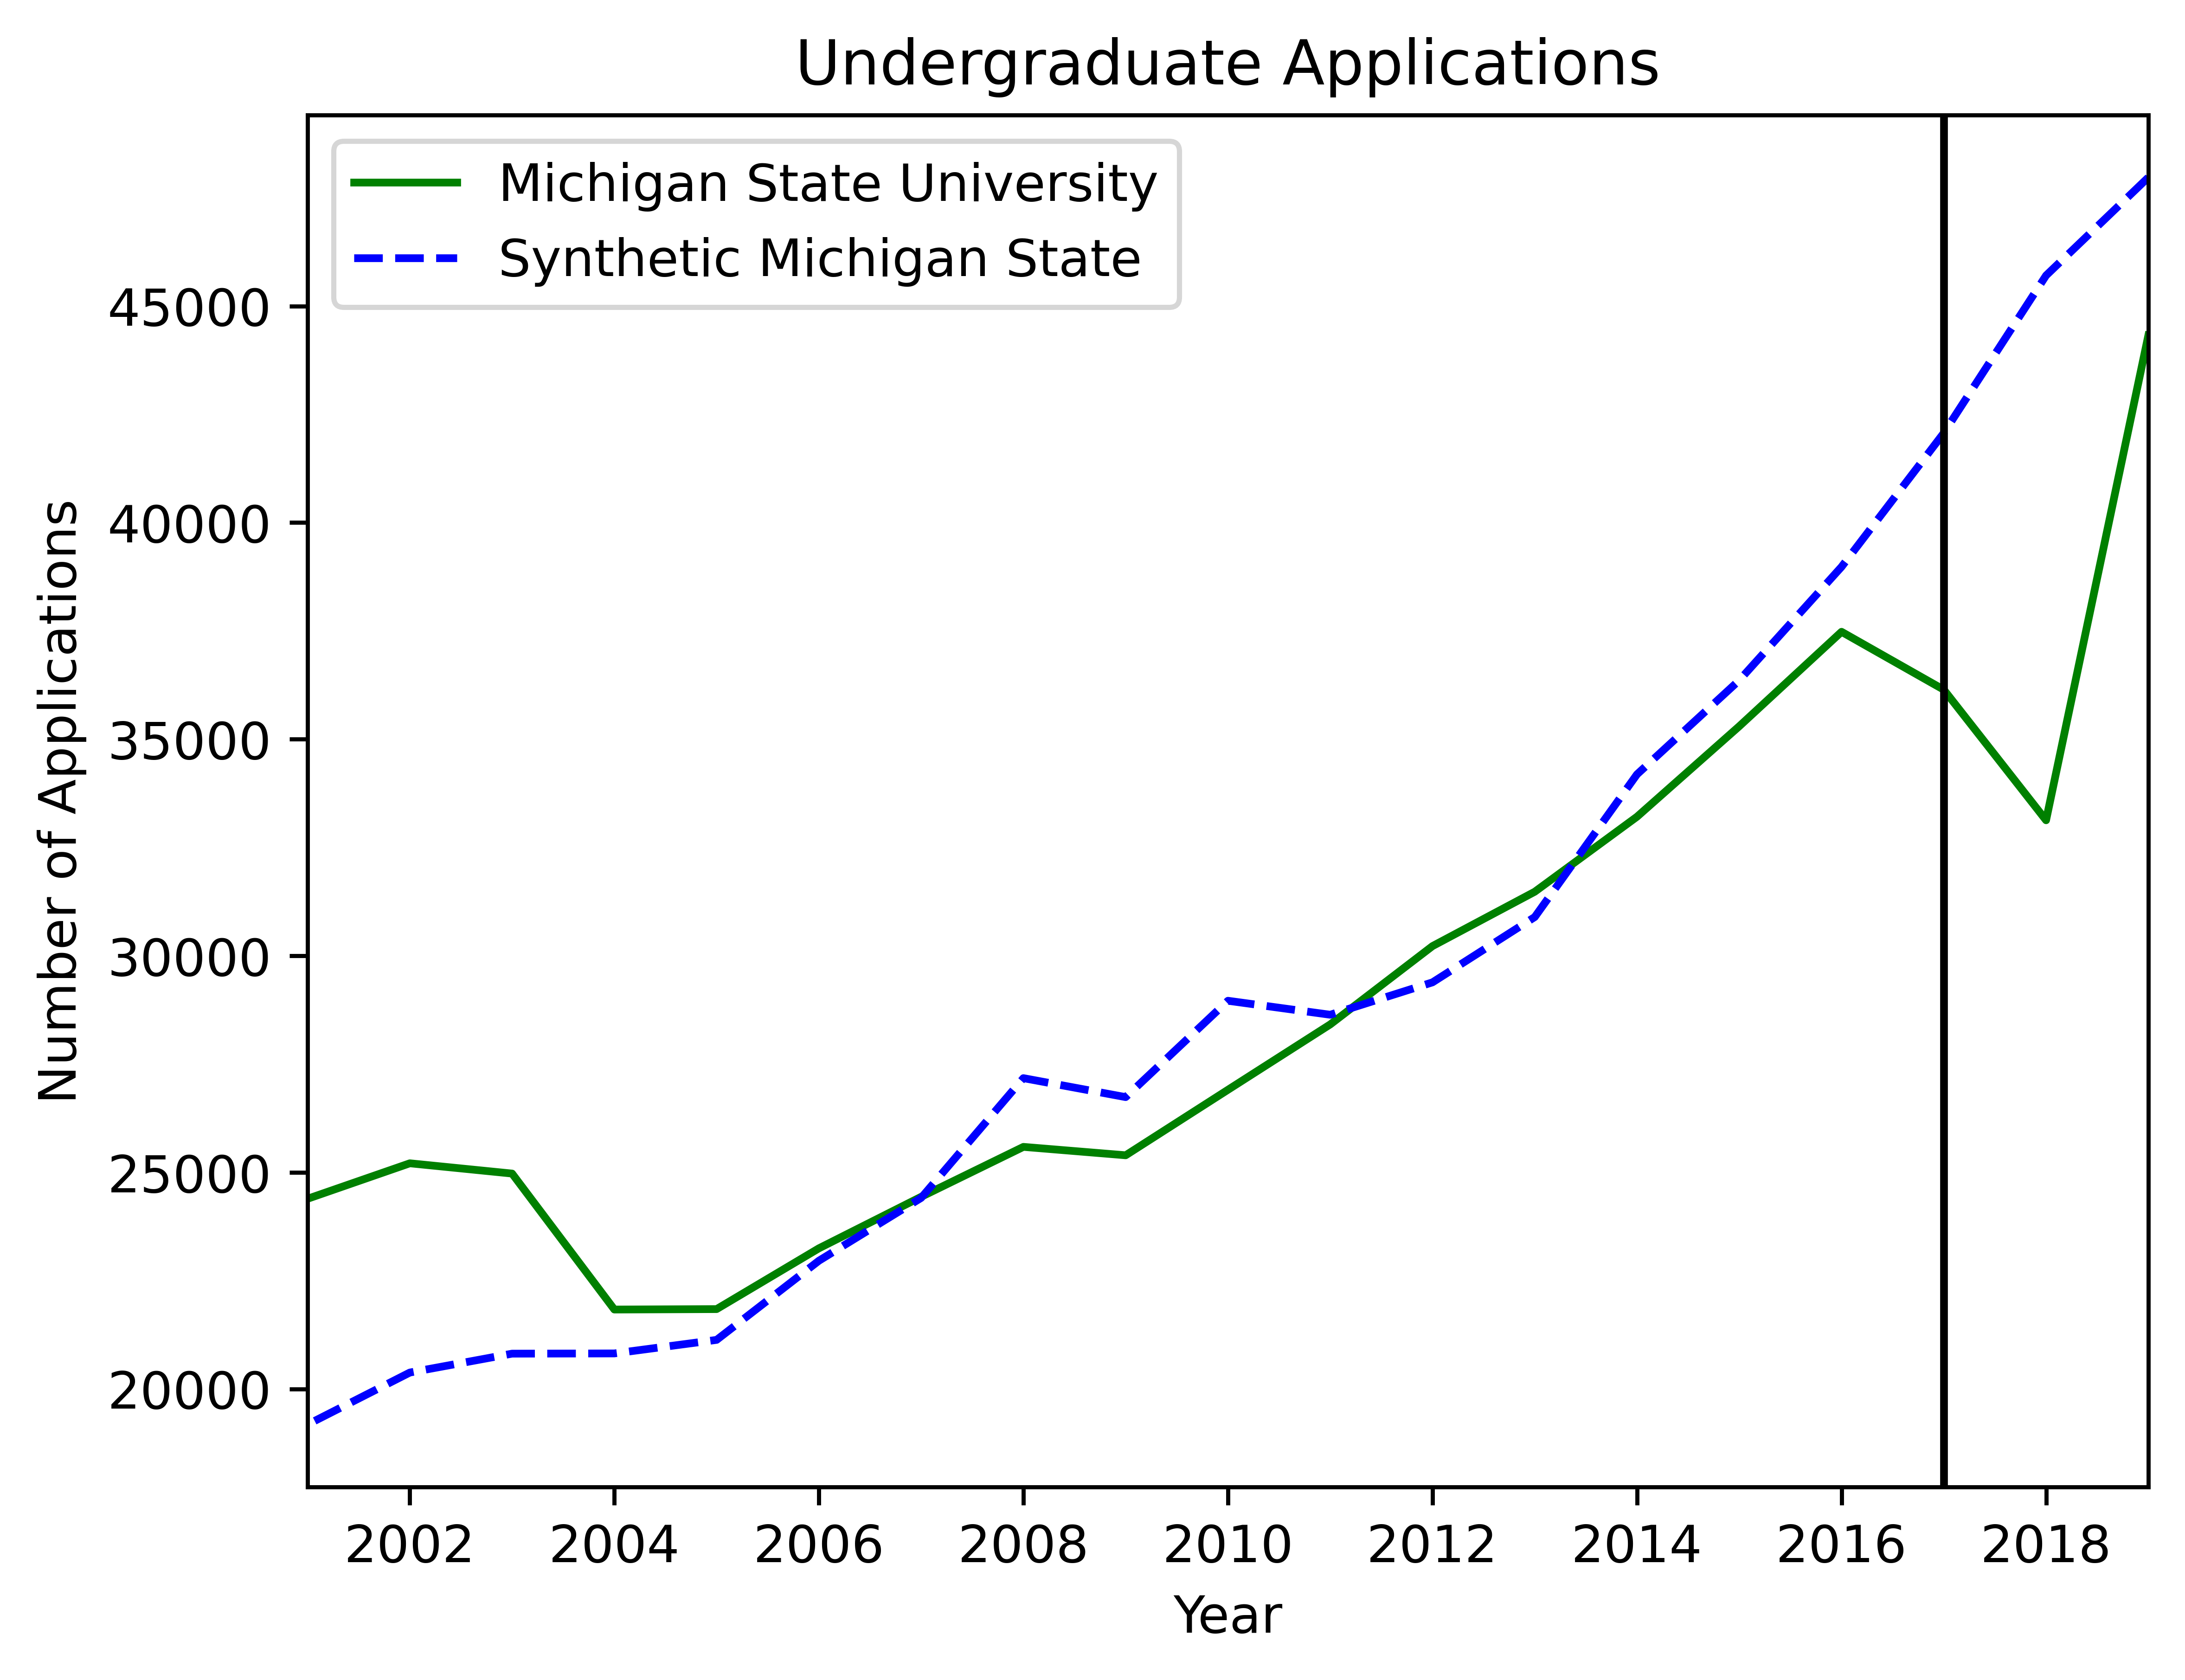
\includegraphics[scale=0.5]{msu_apps.png}
		\caption{Undergraduate Applications: \\ Michigan State University vs. Synthetic}}
\end{figure}
\pagebreak

\noindent A vital part of using a synthetic control method is having enough \enquote{donors} in the donor pool to make up the synthetic control group. As mentioned, we have over 100 schools to accomplish this task, and unlike other studies, we created a new synthetic for every outcome variable of interest. This is because we had a unique problem of our initial synthetic not fitting the pre-trends of each outcome variable, which we know is needed. Given we now have 8 different synthetics, obviously each of these is going to be composed of different schools with varying weights. But in particular, when creating the synthetic for the 75th Percentile SAT Reading Scores, our code had weighted Penn State University as almost 75-percent of the \enquote{Synthetic} Michigan State. Our other synthetics do not have any schools weighted nearly as high. With this weight, we would then expect the statistics for these schools to be almost identical. Plotting this data in a double bar chart, we see very similar statistics as expected.

\begin{figure}[h]
	{\centering
		\captionsetup{justification=centering}
		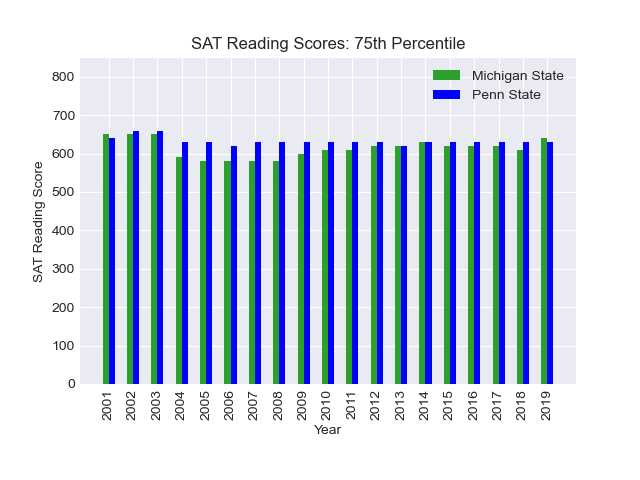
\includegraphics[scale=0.75]{msu_psu_read75pct.png}
		\caption{SAT Reading Scores, 75th Percentile: \\ Michigan State University vs. Penn State University}}
\end{figure}
\pagebreak

\noindent While not entirely related to this project, I was curious which schools had the highest number of applications. (I also wanted to use different kinds of visualizations to become familiar with them.) I used the data set to sort the number of applications by year, ranked each year's applications from lowest to highest, and then obtained the top 10 schools with the highest number of applications received in the year 2019. The ranked bar chart displays these findings. 

\begin{figure}[h]
	{\centering
	\captionsetup{justification=centering}
	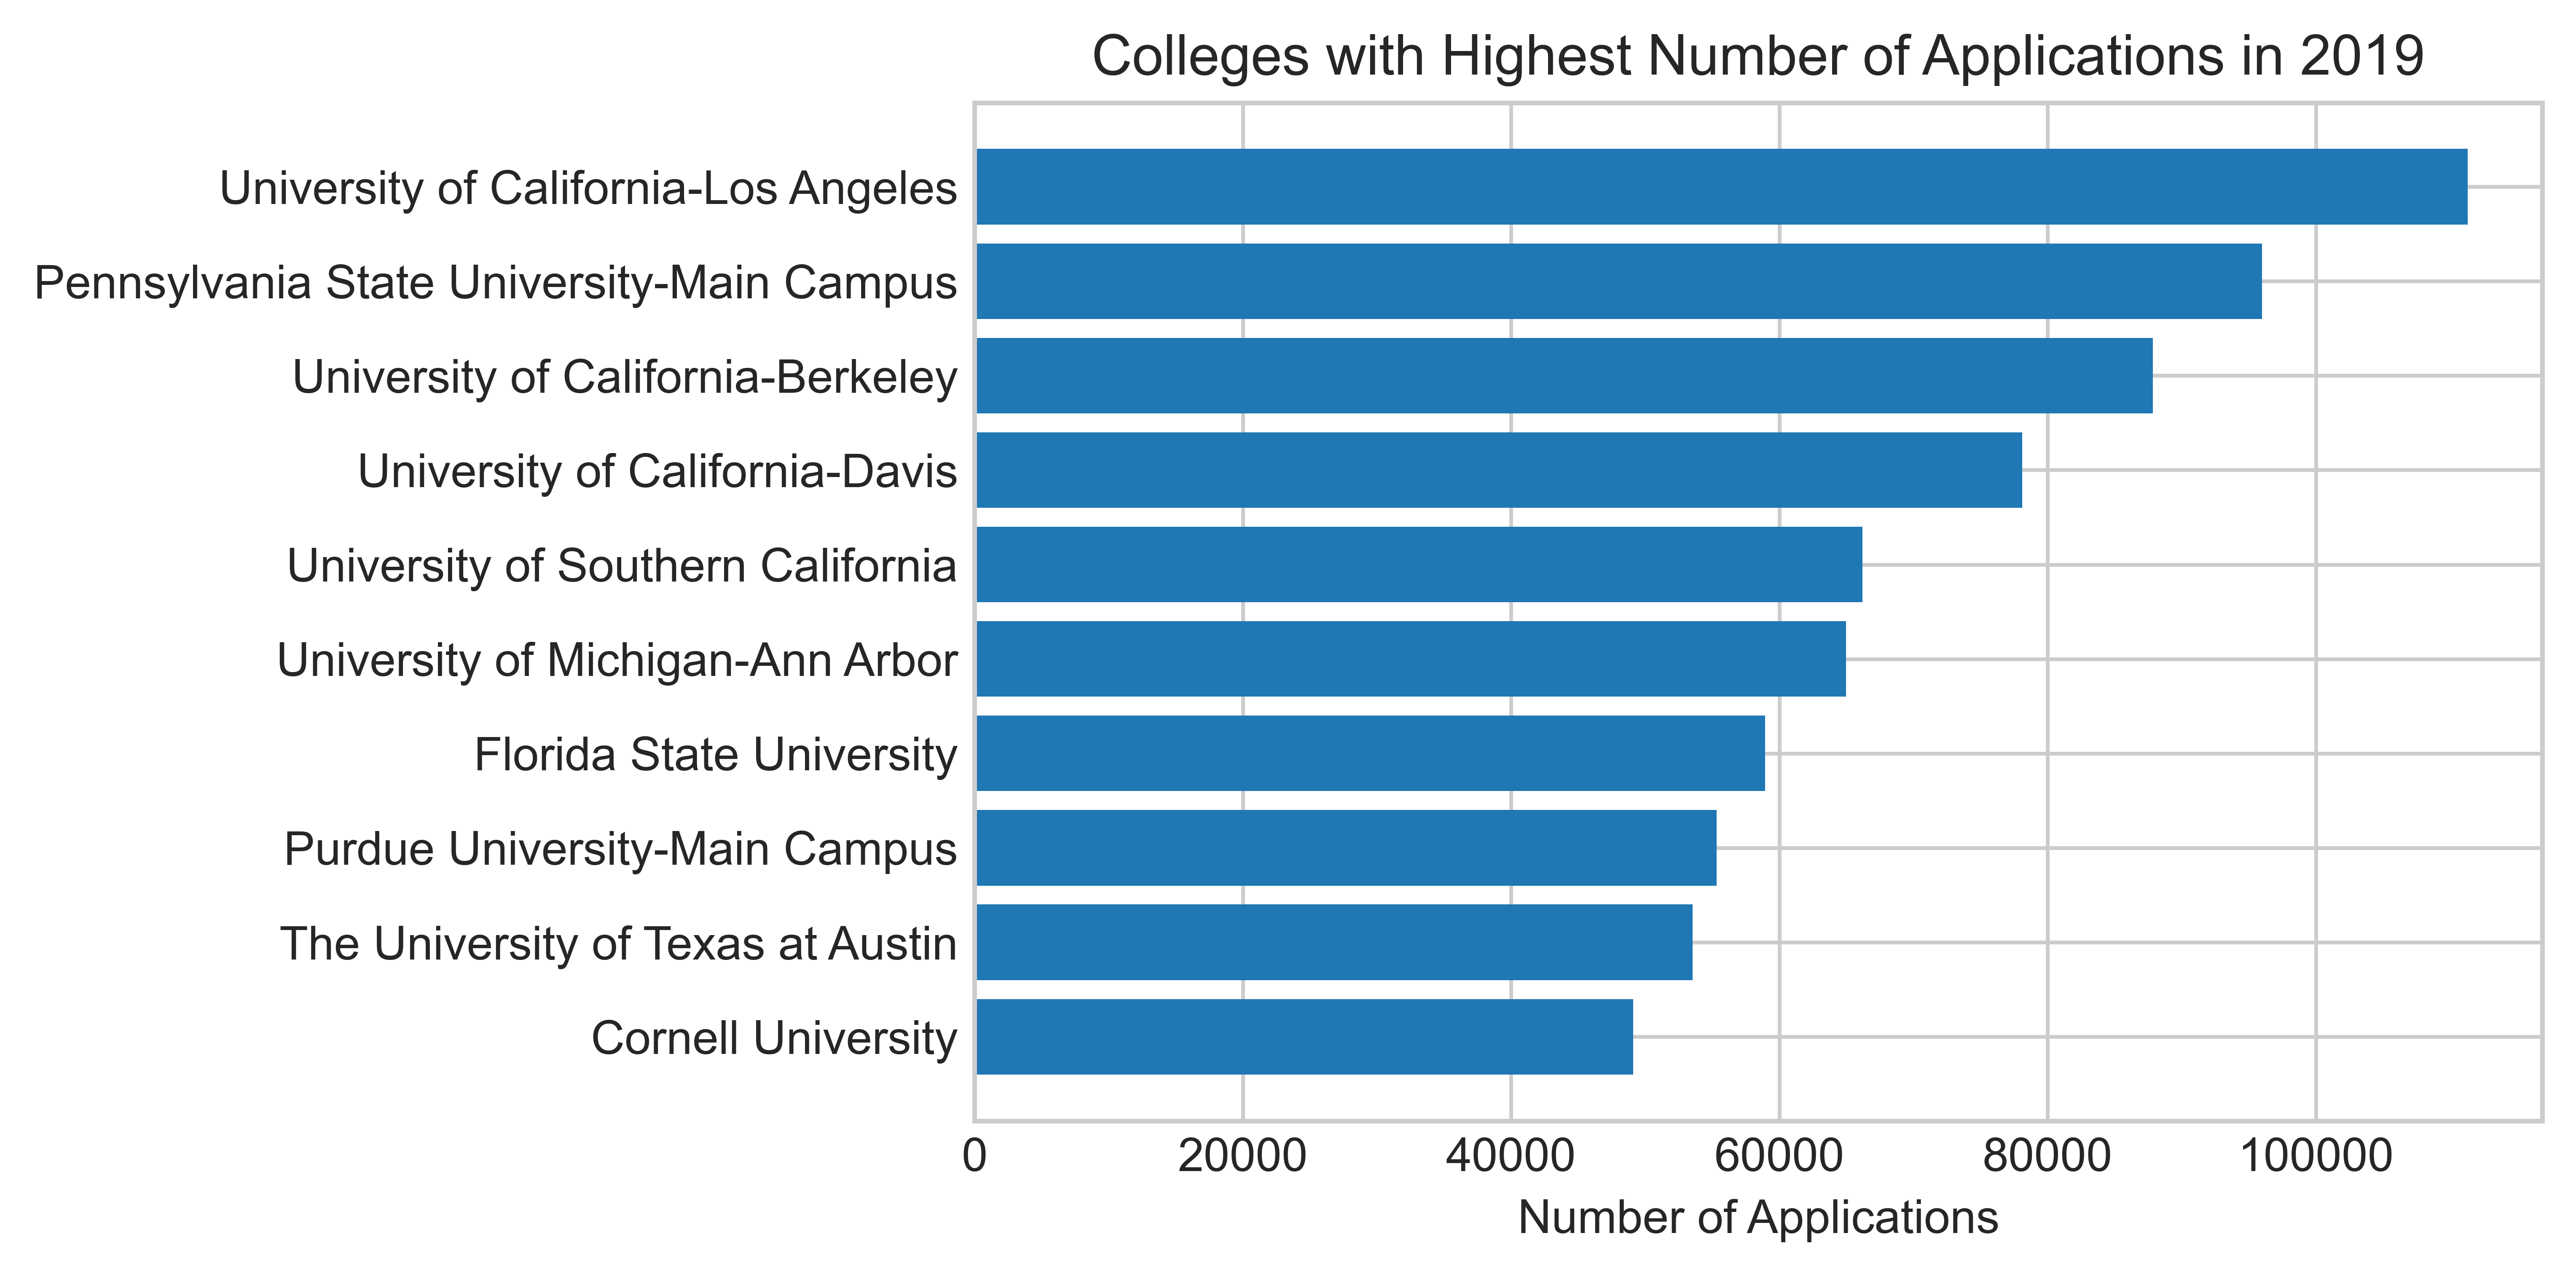
\includegraphics[scale=0.7]{college_apps2.png}
	\caption{2019 Undergraduate Applications: Top 10 Colleges}}
\end{figure}

\end{document}